\documentclass[aspectratio=169]{beamer}

\usepackage[utf8]{inputenc}
\usepackage{amsmath}
\usepackage{amsfonts}
\usepackage{amssymb}
\usepackage{graphicx}
\usepackage{booktabs} % For professional tables
\usepackage{caption}  % Add this line for \captionof command
\usepackage{minted}   % For code highlighting
\usepackage{xcolor}
\usepackage{tikz}  % Add this for TikZ overlays

\setminted{
  breaklines=true,
  % fontsize=\small,
  % fontfamily=pcr,       % Font family: tt (typewriter), zi (Inconsolata), etc.
  % linenos=true,        % line numbers
  % numbersep=5pt,
  % frame=lines,         % frame style: none, leftline, topline, bottomline, lines, single
  framesep=2mm,
  bgcolor=gray!10,      % background color
  tabsize=4,
  autogobble=true,     % auto-remove indentation
  python3=true
}

\bibliographystyle{elsarticle-num-names}

\definecolor{execute_cypher_query}{RGB}{220, 93, 85} % Red-Orange
\definecolor{search_for}{RGB}{212, 219, 93} % Yellow-Green
\definecolor{get_properties_from}{RGB}{78, 222, 94} % Bright Green
\definecolor{get_domains_ranges_of}{RGB}{77, 210, 219} % Cyan
\definecolor{get_components_with_property}{RGB}{89, 87, 222} % Blue-Purple
\definecolor{register_retrieval_result}{RGB}{217, 86, 218} % Pink/Magenta

% % Choose a theme
\usetheme{Antibes}
% \usecolortheme{beaver}

% Adjustments for better presentation
\setbeamertemplate{navigation symbols}{} % Hide navigation symbols
\setbeamertemplate{footline}[frame number] % Show page number
\setbeamerfont{frametitle}{size=\large}
\setbeamerfont{title}{size=\huge}
\setbeamerfont{author}{size=\normalsize}
\setbeamerfont{institute}{size=\small}
\setbeamercovered{transparent} % Make covered items transparent

\title[Text-to-Cypher: An Agentic Approach]{
  Text-to-Cypher: \\
  An Agentic Approach
}
\author{Nicolò Resta}
\institute{University of Bari, Aldo Moro}
% \date{EVALITA 2025}

\begin{document}

% Title Slide
{
  \setbeamercolor{background canvas}{bg=white}
  \begin{frame}
    \titlepage
  \end{frame}
}

% Outline Slide
\begin{frame}
  \frametitle{Outline}
  \tableofcontents
\end{frame}

% --- SECTION 1: INTRODUCTION ---
\section{Introduction \& Motivation}

\begin{frame}{Text-to-Query: The Challenge}
  \begin{itemize}
    \item \textbf{Text-to-Query}: Translating natural language questions into formal database queries.
    \item \textbf{Task}: Bridging the gap between informal natural language and formal languages
    \item \textbf{Goal}: Retrieving structured data from unstructured intent
    \item \textbf{Text-to-Cypher}: A specialized subset for Property Graph Databases.
    \item \textbf{Complexity}:
      \begin{itemize}
        \item Graph structures are complex to express.
        \item Cypher requires "visual" thinking (ASCII art style patterns).
      \end{itemize}
  \end{itemize}
\end{frame}

\begin{frame}{Complexities \& Core Sub-Tasks}
  \begin{enumerate}
    \item \textbf{Relevant Concepts Identification}: Extracting key and relevant concepts such as \textit{entities}, \textit{relationships}, and \textit{properties}.
    \item \textbf{Relevant Formalisms Discovery}: Finding appropriate formal constructs (node labels, relationship types) of the  underlying symbolical framework.
    \item \textbf{Concepts-Formalisms Linking}: Mapping identified concepts to discovered formal constructs (Entity/Relationship/Property Linking).
    \item \textbf{Formalisms Framework Exploitation}: Generating syntactically and semantically correct queries (in Cypher in our case).
  \end{enumerate}

  \begin{block}{Complexity}
    All these sub-tasks are inherently probabilistic or possibilistic in nature.
  \end{block}
\end{frame}

\section{Related Works}

\begin{frame}{Research Landscape: Overview}
    Existing literature splits into two main directions:
    \vspace{0.5cm}
    \begin{enumerate}
        \item \textbf{Benchmark Development}: 
        Creating high-quality datasets for training and evaluation.
        \item \textbf{Text-to-Query Solutions}: 
        Designing architectures (Algorithmic vs. Agentic) to solve the translation task.
    \end{enumerate}
    \vspace{0.5cm}
    \begin{block}{Our Focus}
        We leverage existing benchmarks to propose a novel, zero-shot agentic solution for Text-to-Cypher.
    \end{block}
\end{frame}

\begin{frame}{Research Landscape: Datasets}
    \begin{itemize}
        \item \href{https://huggingface.co/datasets/neo4j/text2cypher-2024v1}{\textbf{neo4j/text2cypher-2024v1}}\footnote{\cite{neo4jlabs-text2cypher-2024}} (Used):
        \begin{itemize}
            \item \textbf{Size}: 44k+ instances (39k train, 4.8k test).
            \item \textbf{Pros}: Access to 17+ live, publicly available Neo4j databases.
            \item \textbf{Relevance}: Enables execution-based evaluation without local setup.
        \end{itemize}
        \vspace{0.5em}
        \item \href{https://huggingface.co/datasets/megagonlabs/cypherbench}{\textbf{megagonlabs/cypherbench}}\footnote{\cite{cypherbench-megagonlabs-2024}} (Excluded):
        \begin{itemize}
            \item \textbf{Size}: ~10k instances (Wikidata derived).
            \item \textbf{Cons}: Requires resource-intensive local deployment via Docker (64-128GB RAM).
            \item \textbf{Relevance}: Too heavy for rapid experimentation.
        \end{itemize}
    \end{itemize}
\end{frame}

\begin{frame}{Incomplete Solutions: The Identification-Discovery-Linking Assumption}
  \begin{itemize}
    \item Most works\footnotemark assume \textbf{Identification}, \textbf{Discovery}, and \textbf{Linking} already solved providing the entire database schema without any \textit{filtering} or \textit{pruning}.

    \item This may lead to excessively large prompts that:
    \begin{itemize}
      \item exceed the model's maximum context window.
      \item pollute context with irrelevant information.
    \end{itemize}

    \item How do systems performs Identification, Discovery, and Linking?
    \begin{itemize}
      \item \textbf{Algorithmic} vs \textbf{Agentic} approaches.
    \end{itemize}
  \end{itemize}
  \footnotetext{
    \cite{dabramo-etal-2025-investigating}\\
    \cite{longwell-etal-2024-triple-augmented}\\
    \cite{cypherbench-megagonlabs-2024}\\
    \cite{neo4jlabs-text2cypher-2024}
  }
\end{frame}

\begin{frame}{Algorithmic Approaches\footnote{\cite{yang-etal-2026-enhancing}}}
  \begin{itemize}
    \item \textbf{Pipeline}: Entity Linking $\rightarrow$ Schema Extraction $\rightarrow$ Generation.
    \item \textbf{Pros}: Deterministic, faster inference, easier to debug.
    \item \textbf{Cons}:
    \begin{itemize}
      \item they rely on strong, domain-specific assumptions that may not generalize
      \item they lack of robust disambiguation mechanisms with multiple candidates
      \item Relationship and Property Linking are often ignored or oversimplified.
    \end{itemize}
  \end{itemize}
\end{frame}

\begin{frame}{Retrieval Architectures: Agentic Approaches\footnote{\cite{grasp-walter-bast-2025,grasp-entity-linking-2025}}}
    \begin{itemize}
      \item \textbf{Loop}: ReAct cycle (Thought $\rightarrow$ Action $\rightarrow$ Observation).
      \item \textbf{Pros}:
      \begin{itemize}
        \item Flexible, adaptable to various domains and tasks.
        \item Can handle ambiguity and multiple candidates through iterative refinement.
      \end{itemize}
      \item \textbf{Cons}: 
      \begin{itemize}
        \item Ensuring Efficiency and Effectiveness at scale remains an open challenge.
        \item Higher latency and potential for loops.
      \end{itemize}
      
    \end{itemize}
\end{frame}

\begin{frame}{Similarity Techniques: The Trade-offs}
    Constraint: Effective retrieval of short schema terms (e.g., DataCenter, founded\_at).
    \begin{itemize}
        \item \textbf{Lexical Matching} (Levenshtein, Jaro-Winkler, Prefix, etc.):
        \begin{itemize}
            \item \textbf{Pros}: Very fast and effective for matching short terms/typos.
            \item \textbf{Cons}: Semantic gaps (Synonyms, Polysemy, etc.).
        \end{itemize}
        % \pause
        \item \textbf{Contextual Dense Embeddings} (BERT-based transformers):
        \begin{itemize}
            \item \textbf{Pros}: Effective for sentence-level semantics.
            \item \textbf{Cons}: Ineffective for very short de-contextualized terms + high compute cost.
        \end{itemize}
        % \pause
        \item \textbf{FastText} (Subword Static Word Embeddings (S-SWEs)):
        \begin{itemize}
            \item \textbf{Pros}: Fast lookup; captures semantics of words/subwords w/o overhead.
            \item \textbf{Cons}: Large memory requirements for storing the vocabulary.
        \end{itemize}
        % \pause
        \item \textbf{Model2Vec}\footnote{\cite{tulkens-2024-model2vec}} (Static Distilled Embeddings) - \textbf{\textit{Our Choice}}:
        \begin{itemize}
            \item \textbf{Pros}: Pros of FastText + memory efficiency
        \end{itemize}
    \end{itemize}
\end{frame}

\section{Proposed Approach}

\begin{frame}{System Architecture}
  \begin{columns}
    \column{0.5\textwidth}
      \begin{itemize}
        \item \textbf{Framework}: LangChain \& LangGraph.
        \item \textbf{Core Engine}: GPT-4.1 (Zero-Shot).
        \item \textbf{Indexing Strategy}:
          \begin{itemize}
            \item \textbf{Vector Store}: FAISS with Model2Vec (\href{https://huggingface.co/minishlab/potion-retrieval-32M}{potion-retrieval-32M}\footnotemark). Indexes Node Labels, Relationship Types, Property Keys.
            \item \textbf{Schema Index}: Inverted index for structural lookups (e.g., node-property mappings).
          \end{itemize}
      \end{itemize}
    \column{0.5\textwidth}
      \begin{figure}
        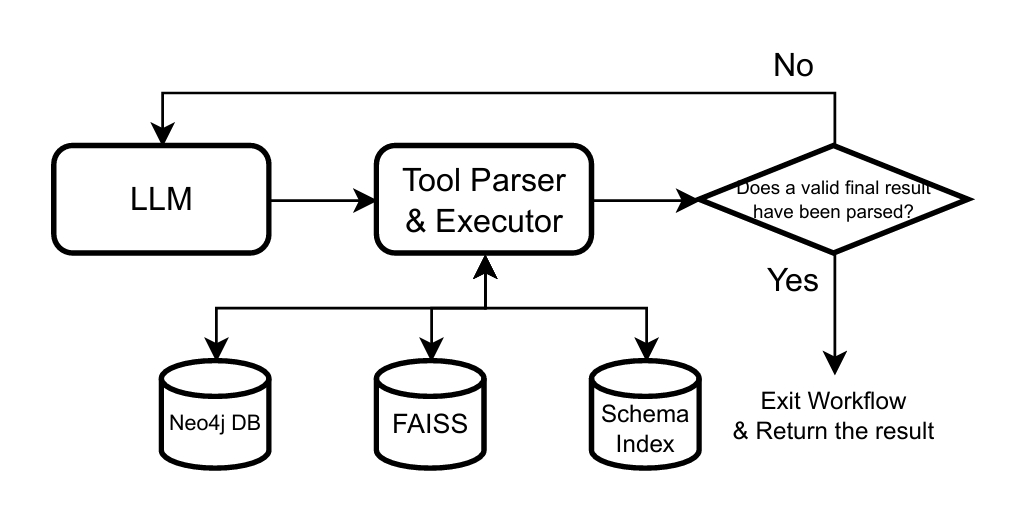
\includegraphics[width=\linewidth]{./rsc/architecture.png}
        \caption{System Architecture}
      \end{figure}
  \end{columns}
  \footnotetext{which is a finetuned version of the \href{https://huggingface.co/minishlab/potion-base-32M}{potion-base-32M}}
\end{frame}

\begin{frame}[fragile]{Tool Design: Semantic Discovery}
  \begin{minted}{python}
  def search_for(
      components: List[Literal["nodes", "relationships", "properties"]],
      similar_to: str,
      top_k: int = 10
  ) -> str:
  \end{minted}
\vspace{0.5em}
\begin{itemize}
    \item \textbf{Purpose}: Semantic search over indexed schema components (FAISS + Model2Vec).
    \item \textbf{Strategy}: Prioritizes \textit{Recall} over Precision to cast a wide initial net.
    \item \textbf{Usage}: Invoked efficiently in parallel for independent concepts in the user query.
\end{itemize}
\end{frame}

\begin{frame}[fragile]{Tool Design: Property Retrieval}
  \begin{minted}{python}
  def get_properties_from(
      components: List[Literal["nodes", "relationships"]],
      of_types: List[str],
      similar_to: Optional[List[str]] = None,
      top_k: Union[int, List[int]] = 10
  ) -> str:
  \end{minted}
\vspace{0.5em}
\begin{itemize}
    \item \textbf{Purpose}: Retrieves properties for explicit node labels or relationship types.
    \item \textbf{Batching}: Processes multiple components in a single call to reduce LLM turns.
    \item \textbf{Context}: Allows filtering property lists by semantic relevance (Model2Vec).
\end{itemize}
\end{frame}

\begin{frame}[fragile]{Tool Design: Structure Exploration}
  \begin{minted}{python}
  def get_domains_ranges_of(
      relationships: List[str],
      similar_to: Optional[List[str]] = None,
      order_by: List[Literal["domains", "ranges"]] = None,
      top_k: Union[int, List[int]] = 10
  ) -> str:
  \end{minted}
\vspace{0.5em}
\begin{itemize}
    \item \textbf{Purpose}: Discovers valid Source (Domain) and Target (Range) nodes for relationships.
    \item \textbf{Graph Traversal}: essential for constructing valid path expressions.
    \item \textbf{Filtering}: Can prioritize certain domains/ranges based on semantic similarity to query concepts (Model2Vec).
\end{itemize}
\end{frame}

\begin{frame}[fragile]{Tool Design: Reverse Lookup}
  \begin{minted}{python}
  def get_components_with_property(
      keys: List[str],
      components: List[Literal["nodes", "relationships", "both"]],
      similar_to: Optional[List[str]] = None,
      top_k: Union[int, List[int]] = 10
  ) -> str:
  \end{minted}
\vspace{0.5em}
\begin{itemize}
    \item \textbf{Purpose}: Finds schema components that possess specific property keys.
    \item \textbf{Disambiguation}: Uses discriminative properties (e.g., \texttt{created\_at}, \texttt{isbn}) to filter candidate types.
    \item \textbf{Mechanism}: Leveraging the inverted schema index for efficient reverse lookups.
\end{itemize}
\end{frame}

\begin{frame}[fragile]{Tool Design: Grounding \& Validation}
  \begin{minted}{python}
  def execute_cypher_query(cypher: str) -> List[dict]:
  \end{minted}
  \vspace{0.5em}
\begin{itemize}
    \item \textbf{Purpose}: Executes arbitrary Cypher queries against the live database.
    \item \textbf{Grounding}: Validates schema assumptions against actual data instances.
    \item \textbf{Data Exploration}: Checks for specific patterns, value formats, or edge cases.
\end{itemize}
\end{frame}

\begin{frame}[fragile]{Tool Design: Result Registration}
  \begin{minted}{python}
  def register_retrieval_result(
      motivation: str,
      cypher_query: Optional[str] = None,
      kg_schema: Optional[KGSchema] = None
  ) -> RetrievalAgent.Result:
  \end{minted}
\vspace{0.5em}
\begin{itemize}
    \item \textbf{Purpose}: Signals the completion of the ReAct loop.
    \item \textbf{Output}: Returns specific structured data (Motivation, Query, Schema Subgraph).
    \item \textbf{Integration}: Passes the final result to the downstream execution system.
\end{itemize}
\end{frame}

\section{Experiments \& Results}

\begin{frame}{Experimental Setup}
    \begin{itemize}
        \item \textbf{Dataset}: Subset of \href{https://huggingface.co/datasets/neo4j/text2cypher-2024v1}{text2cypher-2024v1} (2,471 instances with live DBs).
        \item \textbf{Metrics}:
          \begin{itemize}
            \item \textbf{Result Similarity (RS)}: Jaccard similarity of result sets.
            \item \textbf{Exact Match (EM)}: RS = 1.0.
            \item \textbf{Success Rate}: Completion without exceptions or loops.
            \item \textbf{Provenance Subgraph Jaccard Similarity (PSJS)}: Jaccard similarity of retrieved schema subgraph vs gold schema subgraph.
          \end{itemize}
        \item \textbf{Baselines}: Comparison with Zero-shot and Fine-tuned GPT-4o (from Neo4j Labs paper).
    \end{itemize}
\end{frame}

\begin{frame}{Effectiveness Results}
  Comparison with best baselines of Neo4j-Labs Team\footnote{\cite{neo4jlabs-text2cypher-2024}}. \\
  Our zero-shot agent matches fine-tuned performance.
  \begin{table}
    \centering
    \begin{tabular}{lcccc}
        \hline
        Model & Result Sim. & Exact Match & PSJS & Success Rate \\
        \hline
        GPT-4o (zero-shot) & - & $31.73\%$ & - & - \\
        GPT-4o (fine-tuned) & - & $32.50\%$ & - & - \\
        \textbf{GPT-4.1 (Ours)}  & $\mathbf{41.22\%}$ & $\mathbf{32.62\%}$ & $\mathbf{69.37\%}$ & $89.11\%$ \\
        \hline
    \end{tabular}
  \end{table}
\end{frame}

\begin{frame}{Efficiency Analysis: Absolute Tool Parallelism}
  \begin{table}
    \resizebox{\textwidth}{!}{
      \begin{tabular}{lccccccc}
          \hline
          \textbf{Tool} & \textbf{Mean} & \textbf{Std} & \textbf{Mode} & \textbf{Min} & \textbf{Median} & \textbf{Max} & \textbf{Count} \\
          \hline
          \textcolor{execute_cypher_query}{\rule{8pt}{4pt}} execute\_cypher\_query                      & 1.01 & 0.10 & 1 & 1 & 1 & 4  & 4342 \\
          \textcolor{search_for}{\rule{8pt}{4pt}} search\_for                                            & 3.69 & 1.43 & 4 & 1 & 4 & 11 & 2614 \\
          \textcolor{get_properties_from}{\rule{8pt}{4pt}} get\_properties\_from                        & 1.42 & 0.76 & 1 & 1 & 1 & 16 & 3813 \\
          \textcolor{get_domains_ranges_of}{\rule{8pt}{4pt}} get\_domains\_ranges\_of                  & 1.46 & 0.90 & 1 & 0 & 1 & 12 & 1924 \\
          \textcolor{get_components_with_property}{\rule{8pt}{4pt}} get\_components\_with\_property    & 2.05 & 1.47 & 1 & 1 & 2 & 9  & 523  \\
          \textcolor{register_retrieval_result}{\rule{8pt}{4pt}} register\_retrieval\_result            & 1.00 & 0.00 & 1 & 1 & 1 & 1  & 4659 \\
          \hline
      \end{tabular}
    }
  \end{table}
\end{frame}

\begin{frame}{Efficiency Analysis: Turn Parallelism and Distribution}
  \begin{columns}
    \column{0.5\textwidth}
      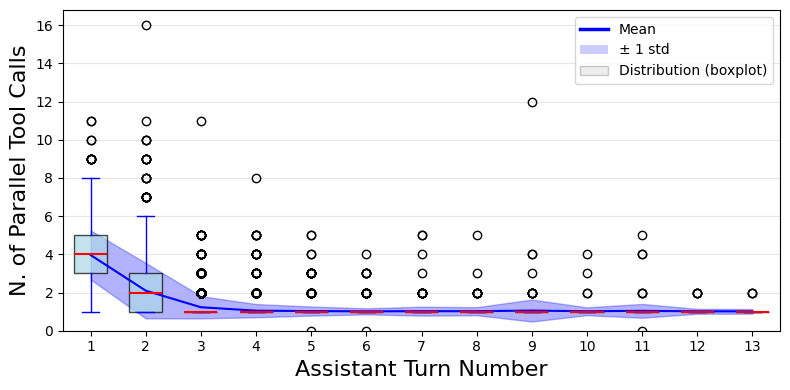
\includegraphics[width=\linewidth]{./rsc/df-parallelism-distribution-over-time.png}
    \column{0.5\textwidth}
      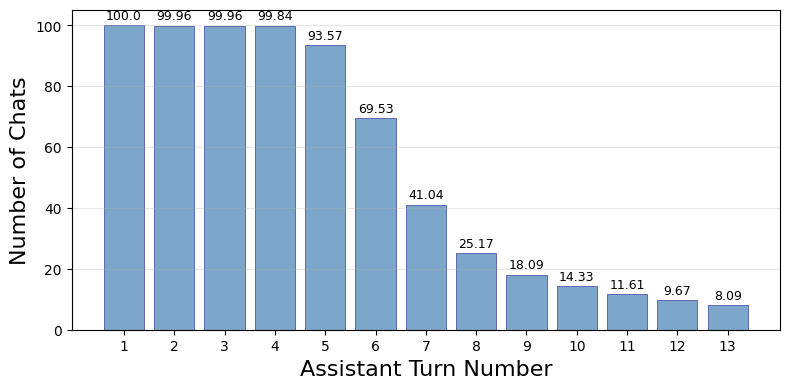
\includegraphics[width=\linewidth]{./rsc/df-ai-turns-distribution.png}
  \end{columns}
\end{frame}

\begin{frame}{Efficiency Analysis: Tool Calls and Errors Distributions}
  \begin{columns}
    \column{0.5\textwidth}
      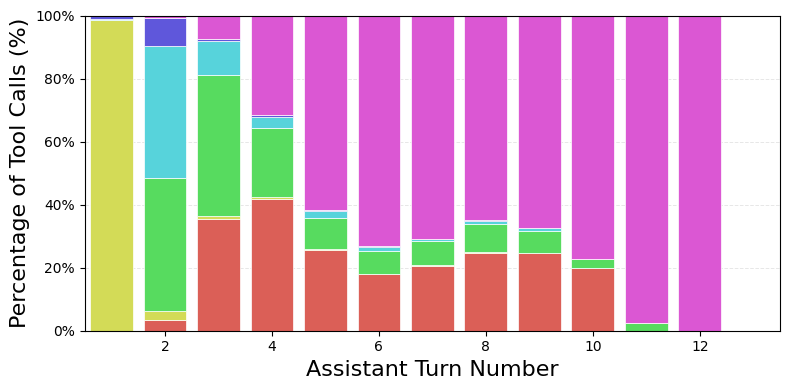
\includegraphics[width=\linewidth]{./rsc/no_na_df-tool-calls-distribution.png}
      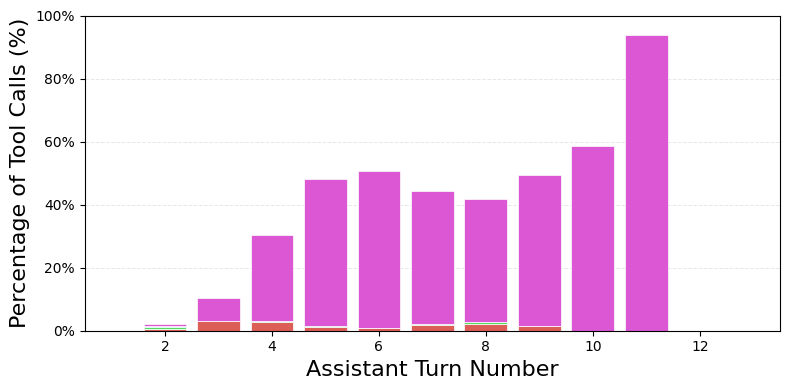
\includegraphics[width=\linewidth]{./rsc/no_na_df-errors-distribution.png}
    \column{0.5\textwidth}
      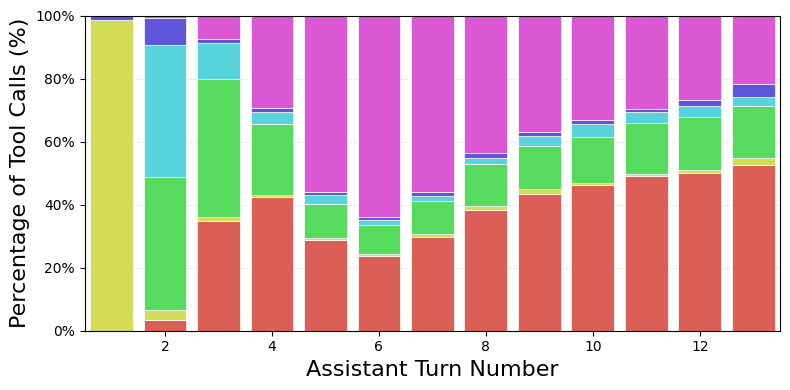
\includegraphics[width=\linewidth]{./rsc/df-tool-calls-distribution.png}
      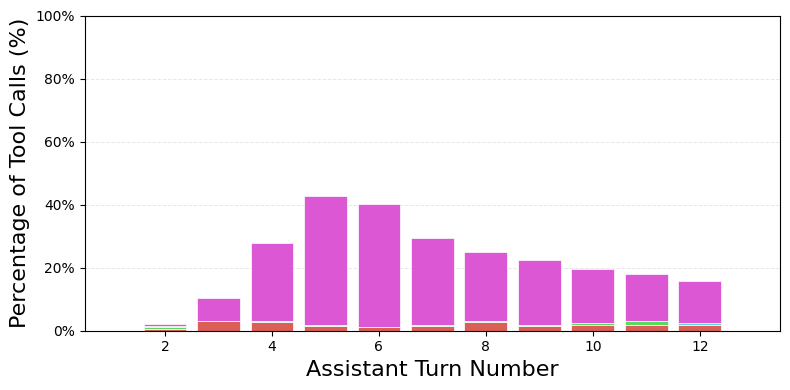
\includegraphics[width=\linewidth]{./rsc/df-errors-distribution.png}
  \end{columns}
  \begin{tikzpicture}[remember picture, overlay]
    \node[anchor=center, yshift=-0.75cm] at (current page.center) {
      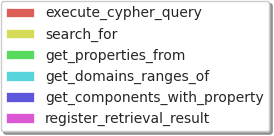
\includegraphics[width=0.25\textwidth]{./rsc/tool-calls-distribution-legend.png}
    };
  \end{tikzpicture}
\end{frame}

\section{Conclusions}

\begin{frame}{Conclusions}
  \begin{itemize}
    \item \textbf{Agentic Approach}: Successfully bridges NL and formal queries without fine-tuning.
    \item \textbf{Performance}: Matches fine-tuned baselines (EM $\approx 32.6\%$).
    \item \textbf{Strategy}: Validated "search-then-refine" behavior with high initial parallelism.
    \item \textbf{Limitations}:
      \begin{itemize}
        \item Struggle with complex, non-linear reasoning paths (backtracking).
        \item JSON formatting errors in final result registration.
      \end{itemize}
    \item \textbf{Future Work}:
      \begin{itemize}
        \item Robust error recovery mechanisms.
        \item Hybrid Fine-tuning for tool usage and formatting.
      \end{itemize}
  \end{itemize}
\end{frame}

\begin{frame}
  \centering
  \Huge Thank You! \\
  \vspace{1cm}
  \normalsize Questions?
  \vspace{0.5cm}
  
  \footnotesize
  \href{mailto:n.resta6@studenti.uniba.it}{n.resta6@studenti.uniba.it} \\
  \url{https://github.com/ashkihotah}
\end{frame}

% include bibliography slide if needed

\bibliography{text-to-cypher}

\end{document}